\documentclass[letterpaper,11pt]{article}
\usepackage{listings}
\usepackage[pdftex]{graphicx} 
\usepackage[utf8]{inputenc}
%\usepackage[english]{babel}
\usepackage{alltt}
\usepackage{color}
\usepackage{url}
\usepackage[T1]{fontenc}
\usepackage{float}
\usepackage{hyperref}
\usepackage{longtable}
\usepackage{caption}
\usepackage{spverbatim}
\usepackage[table,xcdraw]{xcolor}
\usepackage{multirow}
\usepackage{amsmath}

\definecolor{dkgreen}{rgb}{0,0.6,0}
\definecolor{gray}{rgb}{0.5,0.5,0.5}
\definecolor{mauve}{rgb}{0.58,0,0.82}
\definecolor{codegreen}{rgb}{0,0.6,0}
\definecolor{codegray}{rgb}{0.5,0.5,0.5}
\definecolor{codepurple}{rgb}{0.58,0,0.82}
\definecolor{backcolour}{rgb}{0.95,0.95,0.92}

\addtolength{\textwidth}{4cm}
\addtolength{\hoffset}{-2cm}
\addtolength{\textheight}{4cm}
\addtolength{\voffset}{-2cm}

\lstdefinestyle{mystyle}{
    backgroundcolor=\color{backcolour},   
    commentstyle=\color{codegreen},
    keywordstyle=\color{magenta},
    numberstyle=\tiny\color{codegray},
    stringstyle=\color{codepurple},
    basicstyle=\footnotesize,
    breakatwhitespace=false,         
    breaklines=true,                 
    captionpos=b,                    
    keepspaces=true,                 
    numbers=left,                    
    numbersep=5pt,                  
    showspaces=false,                
    showstringspaces=false,
    showtabs=false,                  
    tabsize=2
}

\lstset{style=mystyle}

\lstset{
	basicstyle=\footnotesize,
	breaklines=true,
}

\title{Bibliography management: BibTeX}
\author{Share\LaTeX}

\begin{document}

\begin{titlepage}

\begin{center}

\Huge{Assignment 4}

\Large{CS834-F16:  Introduction to Information Retrieval}

\Large{Fall 2016}


\Large{Erika Siregar}

\vfill

% Bottom of the page
\Large{CS Department - Old Dominion University  \\ \today}


\end{center}

\end{titlepage}


\section*{Question 8.3}
\begin{spverbatim}
For one query in the CACM collection (provided at the book website), generate a ranking using Galago, and then calculate average precision, NDCG at 5 and 10, precision at 10, and the reciprocal rank by hand.
\end{spverbatim}

\subsection*{Answer}
For this assignment, I choose the query no. 3: `intermediate languages used in construction of multi targeted compilers  tcoll'. This query is taken from CACM collection that is available at \url{http://www.search-engines-book.com/collections/}. Based on this query, I generate a ranking using Galago 3.10 \cite{galago_3.10}. I took the top 10 rank positions and follow the guide from the textbook \cite{Croft:2009:SEI:1516224}. Figure \ref{fig:query3_rank} shows the result of the ranking generated using galago. 

\begin{figure}[H]
	\fbox{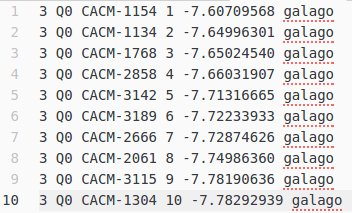
\includegraphics[scale=0.7]{query3_rank}}
	\centering
	\caption{Top 10 Rank Positions for Query no. 3 generated by Galago}
	\label{fig:query3_rank}
\end{figure}

After obtaining this ranking, we are now ready to compute the metrics that are required. In this question, there are 5 metrics that will be calculated:
\begin{enumerate}
	\item Average precision
	\item NDCG at 5
	\item NDCG at 10
	\item Precision at 10
	\item Reciprocal rank
\end{enumerate}

\subsubsection*{Precision, Recall, and Average Precision}
To get the average precision value, we first need to compute recall and precision for each document that is retrieved. Recall is the proportion of relevant documents that are retrieved, and precision is the proportion of retrieved documents that are relevant \cite{Croft:2009:SEI:1516224}. Recall and precision are calculated using these following formulas:
\begin{align}
	Recall = \frac{\left | A \cap B \right |}{\left | A \right |}	 \\
	Precision = \frac{\left | A \cap B \right |}{\left | B \right |}
\end{align}

To get the average precision value, we only need to calculate the average of the precision values from all relevant documents. 

\subsubsection*{NDCG}
Do the following steps to calculate NDCG:
\begin{enumerate}
	\item Set a relevance level for each document. For this assignment, I use boolean code: 1 if the document is relevant and 0 otherwise. 
	\item Calculate the DCG using this formula: 
		\begin{align}
		DCG_p = rel_1 + \sum_{i=2}^p \frac{rel_i}{log_2i}
		\end{align}
		where p is a particular rank \textit{p}, i is the rank for each document, and rel\_i is the relevance level for each document. 
	\item Create the ideal ranks. In my opinion, it is as if we sort the relevance level in the non-increasing order. 
	\item Calculate IDCG in the same way as we do calculation for DCG in point no. 2. 
	\item Finally, calculate NDCG for p = 5 and p = 10 using this formula:
		\begin{align}
		NDCG_p = \frac{DCG_p}{IDCG_p}
		\end{align}
	
\end{enumerate}

\subsubsection*{Precision at 10}
This is similar to the precision that we have discussed in the previous section, but we only consider the precision at rank = 10. 

\subsubsection*{Reciprocal Rank}
Reciprocal rank can be defined as 1 divided by `the rank at which the first relevant document is found'. For example, if the first relevant document is found at rank = 2, then the reciprocal rank is \(\frac{1}{2} \).

Figure \ref{fig:83_query3_metrics} shows the value of average precision, NDCG at 5, NDCG at 10, precision at 10, and the reciprocal rank for query 3. The code to generate this metrics is also can be seen at listing \ref{lst:83}. I also create a library named `galago.py' which is a `wrapper' of Galago tools and also contains the calculation for the metrics that are needed in this assignment. The code for galago.py can be seen on listing \ref{lst:galago.py}

\begin{figure}[H]
	\fbox{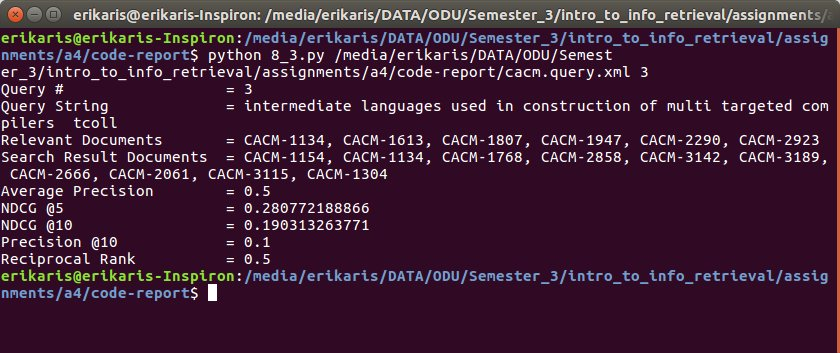
\includegraphics[scale=0.5]{83_query3_metrics}}
	\centering
	\caption{The summary of metrics for query 3}
	\label{fig:83_query3_metrics}
\end{figure}


\begin{lstlisting}[language=python, caption={Code for question 8.3}, label={lst:83}]
#!/usr/bin/python

import errno
import os
from optparse import OptionParser
from lib.galago import GalagoRank

if __name__ == '__main__':
parser = OptionParser(description='Generate a ranking using Galago')
parser.set_usage(parser.get_usage().replace('\n', '') + ' <xml_file_input> [q1 ... qn]')
parser.add_option('-g', '--galago', dest="galago_bin", default='/media/erikaris/DATA/ODU/Semester_3/intro_to_info_retrieval/galago/galago-3.10-bin/bin/galago',
help='Galago "home" directory')
parser.add_option('-d', '--document', dest="document_dir", default='/media/erikaris/DATA/ODU/Semester_3/intro_to_info_retrieval/assignments/a4/code-report/cacm',
help='Document directory to be indexed')
parser.add_option('-j', '--judgements', dest="judgements_file", default='/media/erikaris/DATA/ODU/Semester_3/intro_to_info_retrieval/assignments/a4/code-report/cacm.rel',
help='File .rel as galago eval judgments')
parser.add_option('-r', '--result', dest="result_count", default='10', help='Number of result')

(options, args) = parser.parse_args()
options = vars(options)

if len(args) < 2:
parser.print_help()
exit()


out_dir = os.path.abspath('output')

try: os.makedirs(out_dir)
except OSError, e:
if e.errno != errno.EEXIST: raise

index_dir = os.path.join(os.path.pardir, 'index')
xml_query_file = os.path.abspath(args[0])
json_query_file = os.path.join(out_dir, 'query.json')
rel_file = os.path.join(out_dir, 'result.rel')
res_file = os.path.join(out_dir, 'result.res')
eval_file = os.path.join(out_dir, 'result.eval')

q_ids = []
if len(args) > 1:
q_ids = args[1:]

galago = GalagoRank(options['galago_bin'], options['judgements_file'])
if galago.index(options['document_dir'], index_dir):
for q_id in q_ids:
json_query = galago.build_json_input(xml_query_file, q_id, json_query_file)

rel_docs = galago.get_relevance_docs(q_id)
res_docs = galago.search(index_dir, json_query_file, res_file, options['result_count'])

galago.eval(options['judgements_file'], res_file, eval_file)

print 'Query #                  = {}'.format(json_query['number'])
print 'Query String             = {}'.format(json_query['text'])
print 'Relevant Documents       = {}'.format(', '.join(rel_docs))
print 'Search Result Documents  = {}'.format(', '.join(res_docs))
print 'Average Precision        = {}'.format(galago.get_map(rel_docs, res_docs))
print 'NDCG @5                  = {}'.format(galago.get_ndcg(5, rel_docs, res_docs))
print 'NDCG @10                 = {}'.format(galago.get_ndcg(10, rel_docs, res_docs))
print 'Precision @10            = {}'.format(galago.get_all_precisions(rel_docs, res_docs)[9])
print 'Reciprocal Rank          = {}'.format(galago.get_reciprocal_rank(rel_docs, res_docs))


\end{lstlisting}

\begin{lstlisting}[language=python, caption={Code for galago.py}, label={lst:galago.py}]
#!/usr/bin/python

import json
import os
from math import log
from subprocess import Popen, PIPE, call
from threading import Thread
import xmltodict


class Command(object):
def __init__(self, cmd, out_pipe_callback=None, err_pipe_callback=None):
self.cmd = cmd
self.process = None
self.out_pipe_callback = out_pipe_callback
self.err_pipe_callback = err_pipe_callback

def run(self, timeout, args=()):
def target():
self.process = Popen(self.cmd, stdout=PIPE, stderr=PIPE)

if self.out_pipe_callback:
stdout_thread = Thread(target=self.out_pipe_callback,
args=(self.process.stdout, ) + args)
stdout_thread.daemon = True
stdout_thread.start()

if self.err_pipe_callback:
stderr_thread = Thread(target=self.err_pipe_callback,
args=(self.process.stderr, ) + args)
stderr_thread.daemon = True
stderr_thread.start()

self.process.wait()

thread = Thread(target=target)
thread.daemon = True
thread.start()

thread.join(timeout)
try: self.process.terminate()
except: pass

return self.process.returncode


class GalagoRank(object):
galago_bin = None
rel_docs = {}
res_docs = []

def __init__(self, galago_bin, judgements_file):
self.galago_bin = galago_bin
self.rel_docs = self.build_relevance(judgements_file)

def index(self, document_dir, index_dir):
if not os.path.exists(index_dir):
bash = '"{}" build --indexPath="{}" --inputPath="{}"'.format(
self.galago_bin, index_dir, document_dir)

code = call(['bash', '-c', bash])
return code == 0

else:
return True

def build_relevance(self, judgements_file):
with open(judgements_file, 'r') as fp:
rel_docs = {}
for line in fp.readlines():
q, a, doc, b = line.split()

rel_docs.setdefault(q, [])
rel_docs[q].append(doc)

return rel_docs
return {}

def get_relevance_docs(self, q):
return self.rel_docs[q]

def get_result_docs(self):
return self.res_docs

def build_json_input(self, xml_query_file, id, json_query_file):
json_query = json.dumps(xmltodict.parse(open(xml_query_file).read()))
json_query = json.loads(json_query)
json_query = json_query['parameters']['query']

selected_json_query = {}
selected_json_query.setdefault('query', [])
for query in json_query:
if query['number'] == id:
selected_json_query['query'].append({
'number' : id,
'text' : query['text']
})

open(json_query_file, 'wb').write(json.dumps(selected_json_query))

return selected_json_query['query'][0]

def search(self, index_dir, json_query_file, result_file, count):
res_docs = []

cmd = Command([self.galago_bin, 'batch-search', '--index={}'.format(index_dir),
'--requested={}'.format(count), '{}'.format(json_query_file)],
self.search_result)
cmd.run(60 * 10, args=(res_docs, result_file, ))

return res_docs

def search_result(self, out, res_docs, result_file):
lines = []
if out and hasattr(out, 'readline'):
for line in iter(out.readline, b''):
line = line.strip()
q_id, a, doc, id, score, b = self.search_parse(line)
lines.append((q_id, a, doc, id, score, b))
res_docs.append(doc)

with open(result_file, 'wb') as fp:
fp.write('\n'.join([' '.join(l) for l in lines]))
fp.close()

def search_parse(self, line):
parts = line.split()
if len(parts) == 6:
q_id, a, doc, id, score, b = parts
else:
q_id = parts[0]
a = parts[1]
doc = ' '.join(parts[2:len(parts)-3])
id = parts[len(parts) - 3]
score = parts[len(parts) - 2]
b = parts[len(parts) - 1]

doc = os.path.basename(doc)
doc = os.path.splitext(doc)[0]
return q_id, a, doc, id, score, b

def eval(self, rel_file, res_file, eval_file):
bash = '{} eval --judgments="{}" --baseline="{}" > "{}"'.format(
self.galago_bin, rel_file, res_file, eval_file)

cmd = Command(['bash', '-c', bash])
code = cmd.run(60 * 10)

return code == 0

def get_precision(self, rel_docs, res_docs):
relset = set(rel_docs)
retrset = set(res_docs)

return float(len(relset.intersection(retrset))) / len(retrset)

def get_recall(self, rel_docs, res_docs):
relset = set(rel_docs)
retrset = set(res_docs)

return float(len(relset.intersection(retrset))) / len(relset)

def get_all_precisions(self, rel_docs, res_docs):
rr = []
for i in range(1, len(res_docs) + 1):
rr.append(self.get_precision(rel_docs, res_docs[:i]))

return rr

def get_all_recalls(self, rel_docs, res_docs):
rr = []
for i in range(1, len(res_docs) + 1):
rr.append(self.get_recall(rel_docs, res_docs[:i]))

return rr

def get_map(self, rel_docs, res_docs):
rr = self.get_all_precisions(rel_docs, res_docs)

res = []
for i in range(len(res_docs)):
if res_docs[i] in rel_docs:
res.append(rr[i])

if len(res) == 0:
return 0.0

return float(sum(res)) / len(res)

def get_relevance(self, i, rel_docs, res_docs):
return 1 if res_docs[i] in rel_docs else 0

def get_dcg(self, p, rel_docs, res_docs):
sum = 0
for i in range(2, p + 1):
sum += float(self.get_relevance(i-1, rel_docs, res_docs)) / log(i, 2)
return self.get_relevance(0, rel_docs, res_docs) + sum

def get_idcg(self, p):
sum = 0
for i in range(2, p + 1):
sum += 1 / log(i, 2)
return 1 + sum

def get_ndcg(self, p, rel_docs, res_docs):
dcg = self.get_dcg(p, rel_docs, res_docs)
idcg = self.get_idcg(p)
return dcg / idcg

def get_reciprocal_rank(self, rel_docs, res_docs):
for i in range(1, len(res_docs) + 1):
if res_docs[i - 1] in rel_docs:
return 1.0 / i
return 0.0

\end{lstlisting}



\noindent\makebox[\linewidth]{\rule{\textwidth}{0.4pt}}

\section*{Question 8.4}
\begin{spverbatim}
For two queries in the CACM collection, generate two uninterpolated recall-precision graphs, a table of interpolated precision values at standard recall levels, and the average
interpolated recall-precision graph. 
\end{spverbatim}

\subsection*{Answer:}
For this assignment, I randomly choose query no. 6 and no. 12 and calculate the recall and precision values based on the top 10 rank positions. The code to do this can be seen on listing \ref{lst:84}. To generate the recall-precision graph, I use python library \textit{matplotlib} \cite{matplotlib} based on example from \cite{matplotlib-example}. 
\newline
Figure \ref{fig:84_uninterpolated} and figure \ref{fig:84_interpolated} show the uninterpolated and interpolated recall-precision graphs for query no. 6 and 12. The table of interpolated precision values can be seen in figure 

\begin{figure}[H]
	\fbox{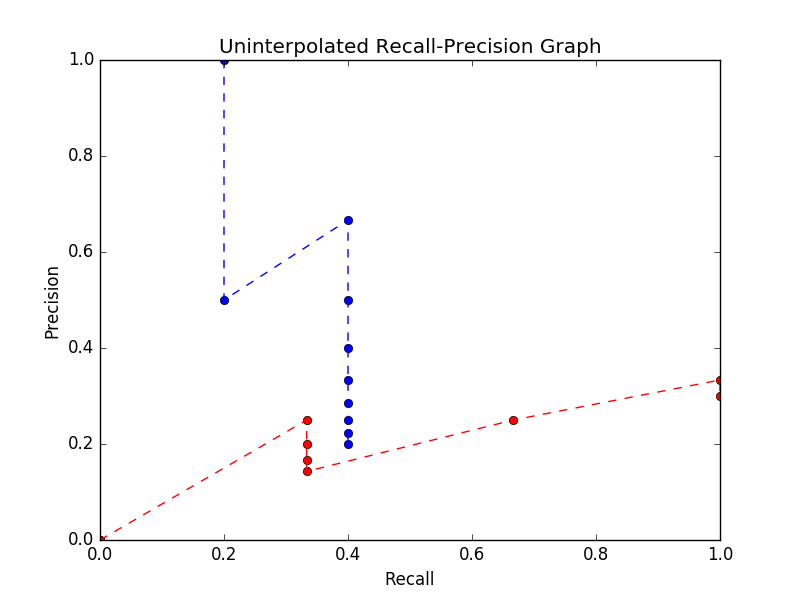
\includegraphics[scale=0.6]{uninterpolated}}
	\centering
	\caption{Uninterpolated recall-precision graph for query no. 6 and 12}
	\label{fig:84_uninterpolated}
\end{figure}

\begin{figure}[H]
	\fbox{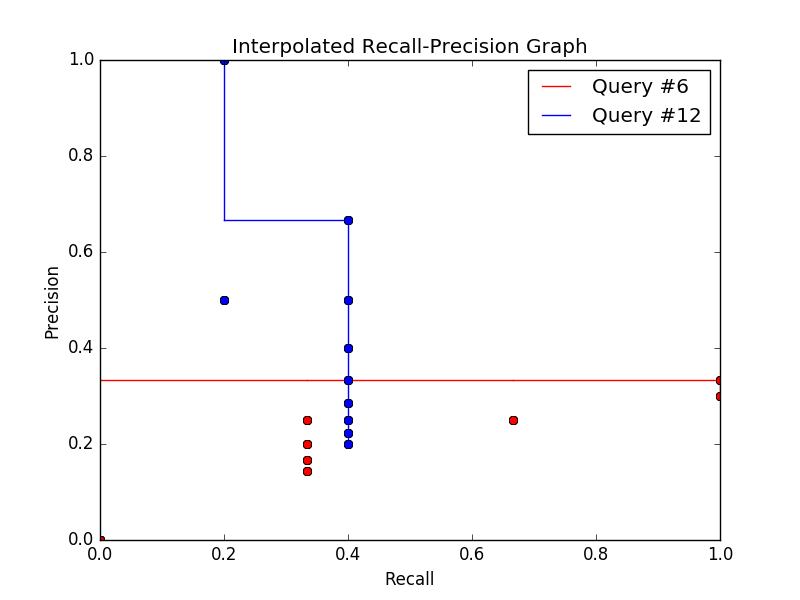
\includegraphics[scale=0.6]{interpolated}}
	\centering
	\caption{Interpolated recall-precision graph for query no. 6 and 12}
	\label{fig:84_interpolated}
\end{figure}

\begin{figure}[H]
	\fbox{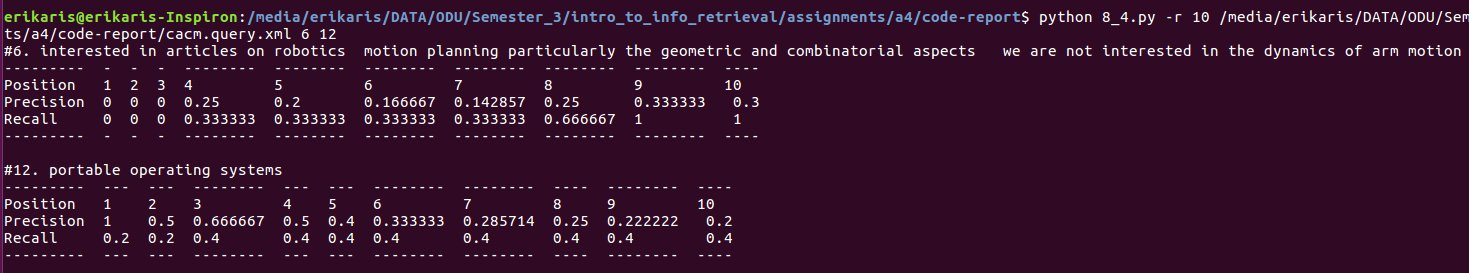
\includegraphics[scale=0.4]{84_query6_12_table}}
	\centering
	\caption{Table of interpolate for query no. 6 and 12}
	\label{fig:84_query6_12_table}
\end{figure}



\begin{lstlisting}[language=python, caption={Code for question 8.4}, label={lst:84}]
#!/usr/bin/python

import os
from optparse import OptionParser

import errno
from tabulate import tabulate
from lib.galago import GalagoRank
import matplotlib.pyplot as plt
import numpy as np

if __name__ == '__main__':
parser = OptionParser(description='Generate a ranking using Galago')
parser.set_usage(parser.get_usage().replace('\n', '') + ' <xml_file_input> [q1 ... qn]')
parser.add_option('-g', '--galago', dest="galago_bin", default='/media/erikaris/DATA/ODU/Semester_3/intro_to_info_retrieval/galago/galago-3.10-bin/bin/galago',
help='Galago "home" directory')
parser.add_option('-d', '--document', dest="document_dir", default='/media/erikaris/DATA/ODU/Semester_3/intro_to_info_retrieval/assignments/a4/code-report/cac',
help='Document directory to be indexed')
parser.add_option('-j', '--judgements', dest="judgements_file", default='/media/erikaris/DATA/ODU/Semester_3/intro_to_info_retrieval/assignments/a4/code-report/cacm.rel',
help='File .rel as galago eval judgments')
parser.add_option('-r', '--result', dest="result_count", default='10', help='Number of result')

(options, args) = parser.parse_args()
options = vars(options)

if len(args) < 2:
parser.print_help()
exit()


out_dir = os.path.abspath('output')

try: os.makedirs(out_dir)
except OSError, e:
if e.errno != errno.EEXIST: raise

index_dir = os.path.join(os.path.pardir, 'index')
xml_query_file = os.path.abspath(args[0])

q_ids = []
if len(args) > 1:
q_ids = args[1:]

recals_precisions = []
galago = GalagoRank(options['galago_bin'], options['judgements_file'])
if galago.index(options['document_dir'], index_dir):
for q_id in q_ids:
json_query_file = os.path.join(out_dir, 'query_{}.json'.format(q_id))
res_file = os.path.join(out_dir, 'result_{}.res'.format(q_id))
eval_file = os.path.join(out_dir, 'result_{}.eval'.format(q_id))

json_query = galago.build_json_input(xml_query_file, json_query_file, q_id)

rel_docs = galago.get_relevance_docs(q_id)
res_docs = galago.search(index_dir, json_query_file, res_file, options['result_count'])

precisions = galago.get_all_precisions(rel_docs, res_docs)
recals = galago.get_all_recalls(rel_docs, res_docs)

recals_precisions.append((recals, precisions))

table = [['Position', ] + range(1, 11)]
table.append(['Precision', ] + precisions)
table.append(['Recall', ] + recals)

print '#{}. {}'.format(json_query['number'], json_query['text'])
print tabulate(table)
print('')


# Uninterpolated
colors = 'rbgcmyk'
for i, (recals, precisions) in enumerate(recals_precisions):
plt.plot(recals, precisions, marker='o', linestyle='None', color=colors[i])
plt.plot(recals, precisions, marker='None', linestyle='--', color=colors[i])

plt.xlabel('Recall')
plt.ylabel('Precision')
plt.title('Uninterpolated Recall-Precision Graph')
plt.savefig(os.path.join(out_dir, 'uninterpolated.png'))
plt.show()
plt.clf()

# Interpolated
# Reference : http://stackoverflow.com/questions/39836953/how-to-draw-a-precision-recall-curve-with-interpolation-in-python
colors = 'rbgcmyk'
for j, (recals, precisions) in enumerate(recals_precisions):
recals = np.asarray(recals)
precisions = np.asarray(precisions)
precisions2 = precisions.copy()

i = recals.shape[0] - 2
while i >= 0:
if precisions[i + 1] > precisions[i]:
precisions[i] = precisions[i + 1]
i = i - 1

for i in range(recals.shape[0] - 1):
plt.plot((recals[i], recals[i]), (precisions[i], precisions[i + 1]), 'k-', label='', color=colors[j])  # vertical
plt.plot((recals[i], recals[i + 1]), (precisions[i + 1], precisions[i + 1]), 'k-', label='', color=colors[j])  # horizontal
# plt.plot(recals, precisions2, 'k--', color=colors[j])

plt.xlabel('Recall')
plt.ylabel('Precision')
plt.title('Interpolated Recall-Precision Graph')
plt.savefig(os.path.join(out_dir, 'interpolated.png'))
plt.show()


\end{lstlisting}


\noindent\makebox[\linewidth]{\rule{\textwidth}{0.4pt}}

\section*{Question 8.5}
\begin{spverbatim}
Generate the mean average precision, recall-precision graph, average NDCG
at 5 and 10, and precision at 10 for the entire CACM query set
\end{spverbatim}

\subsection*{Answer}
The code to solve this problem can be found on listing \ref{lst:85}. Figure \ref{fig:85_metrics} shows the value of mean average precision (MAP), average NDCG at 5 and 10, and precision at 10 for the entire CACM query set. The recall-precision graph is shown in figure \ref{fig:85_recall-precision}.

\begin{figure}[H]
	\fbox{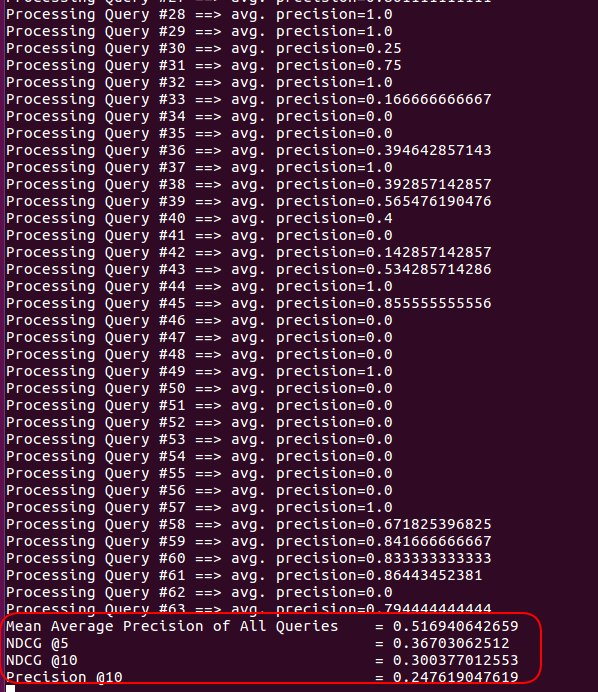
\includegraphics[scale=0.6]{85_metrics}}
	\centering
	\caption{MAP, NDCG at 5 and 10, precision at 10 for the entire CACM query set}
	\label{fig:85_metrics}
\end{figure}

\begin{figure}[H]
	\fbox{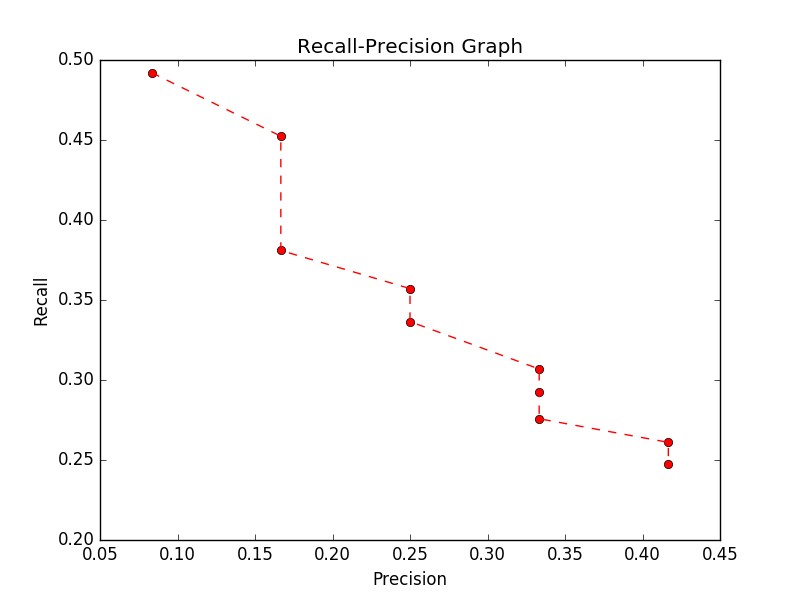
\includegraphics[scale=0.6]{85_recall-precision}}
	\centering
	\caption{Recall-precision graph for the entire CACM query set}
	\label{fig:85_recall-precision}
\end{figure}



\begin{lstlisting}[language=python, caption={Code for question 8.5}, label={lst:85}]
#!/usr/bin/python
import errno
import os
from optparse import OptionParser
import matplotlib.pyplot as plt
import numpy
from lib.galago import GalagoRank

if __name__ == '__main__':
parser = OptionParser(description='Generate a ranking using Galago')
parser.set_usage(parser.get_usage().replace('\n', '') + ' <xml_file_input>')
parser.add_option('-g', '--galago', dest="galago_bin", default='/media/erikaris/DATA/ODU/Semester_3/intro_to_info_retrieval/galago/galago-3.10-bin/bin/galago',
help='Galago "home" directory')
parser.add_option('-d', '--document', dest="document_dir", default='/media/erikaris/DATA/ODU/Semester_3/intro_to_info_retrieval/assignments/a4/code-report/cacm',
help='Document directory to be indexed')
parser.add_option('-j', '--judgements', dest="judgements_file", default='/media/erikaris/DATA/ODU/Semester_3/intro_to_info_retrieval/assignments/a4/code-report/cacm.rel',
help='File .rel as galago eval judgments')
parser.add_option('-r', '--result', dest="result_count", default='10', help='Number of result')

(options, args) = parser.parse_args()
options = vars(options)

if len(args) < 1:
parser.print_help()
exit()


out_dir = os.path.abspath('output')

try: os.makedirs(out_dir)
except OSError, e:
if e.errno != errno.EEXIST: raise

index_dir = os.path.abspath(os.path.join(os.path.pardir, 'index'))
xml_query_file = os.path.abspath(args[0])
json_query_file = os.path.join(out_dir, 'query.json')
rel_file = os.path.join(out_dir, 'result.rel')
res_file = os.path.join(out_dir, 'result.res')
eval_file = os.path.join(out_dir, 'result.eval')

recals_precisions = []
maps = []
ndcg_5s = []
ndcg_10s = []
prec_10s = []
galago = GalagoRank(options['galago_bin'], options['judgements_file'])
if galago.index(options['document_dir'], index_dir):
for q_id in range(1, 64):
json_query_file = os.path.join(out_dir, 'query_{}.json'.format(q_id))
res_file = os.path.join(out_dir, 'result_{}.res'.format(q_id))
eval_file = os.path.join(out_dir, 'result_{}.eval'.format(q_id))

json_query = galago.build_json_input(xml_query_file, json_query_file, q_id)

rel_docs = galago.get_relevance_docs(q_id)
res_docs = galago.search(index_dir, json_query_file, res_file, options['result_count'])

precisions = galago.get_all_precisions(rel_docs, res_docs)
recals = galago.get_all_recalls(rel_docs, res_docs)

map = galago.get_map(rel_docs, res_docs)
maps.append(map)
ndcg_5s.append(galago.get_ndcg(5, rel_docs, res_docs))
ndcg_10s.append(galago.get_ndcg(10, rel_docs, res_docs))
prec_10s.append(galago.get_all_precisions(rel_docs, res_docs)[9])

recals_precisions.append((recals, precisions))

print 'Processing Query #{} ==> avg. precision={}'.format(q_id, map)

# Calculate avg of map
print 'Mean Average Precision of All Queries    = {}'.format(float(sum(maps)) / len(maps))
print 'NDCG @5                                  = {}'.format(float(sum(ndcg_5s)) / len(ndcg_5s))
print 'NDCG @10                                 = {}'.format(float(sum(ndcg_10s)) / len(ndcg_10s))
print 'Precision @10                            = {}'.format(float(sum(prec_10s)) / len(prec_10s))

# Graph
# Transpose
recals_precisions = numpy.asarray(recals_precisions).T.tolist()

recalls = []
precisions = []
for d_recalls, d_precisions in recals_precisions:
recalls.append(float(sum(d_recalls)) / len(d_recalls))
precisions.append(float(sum(d_precisions)) / len(d_precisions))

plt.plot(recals, precisions, marker='o', linestyle='None', color='r')
plt.plot(recals, precisions, marker='None', linestyle='--', color='r')

plt.xlabel('Precision')
plt.ylabel('Recall')
plt.title('Recall-Precision Graph')
plt.savefig(os.path.join(out_dir, 'recall-precision.png'))
plt.show()
plt.clf()


\end{lstlisting}



\noindent\makebox[\linewidth]{\rule{\textwidth}{0.4pt}}

\section*{Question 8.7}
\begin{spverbatim}
Another measure that has been used in a number of evaluations is R-precision.
This is defined as the precision at R documents, where R is the number of relevant
documents for a query. It is used in situations where there is a large variation in
the number of relevant documents per query. Calculate the average R-precision
for the CACM query set and compare it to the other measures.
\end{spverbatim}

\subsection*{Answer}
The script to calculate R-precision can be seen in listing \ref{lst:87}. Figure \ref{fig:87_output} shows the comparison between R-precision and other evaluation metrics for the entire CACM query set. 

\begin{figure}[H]
	\fbox{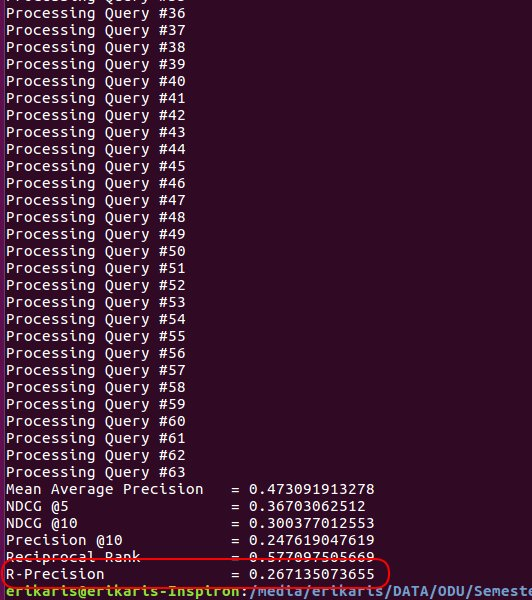
\includegraphics[scale=0.6]{87_output}}
	\centering
	\caption{R-precision and other evaluation measures for the entire CACM query set}
	\label{fig:87_output}
\end{figure}

\begin{lstlisting}[language=python, caption={Script for calculating R-precision}, label={lst:87}]
#!/usr/bin/python

import errno
import os
from optparse import OptionParser
from lib.galago import GalagoRank

if __name__ == '__main__':
parser = OptionParser(description='Generate a ranking using Galago')
parser.set_usage(parser.get_usage().replace('\n', '') + ' <xml_file_input>')
parser.add_option('-g', '--galago', dest="galago_bin", default='/media/erikaris/DATA/ODU/Semester_3/intro_to_info_retrieval/galago/galago-3.10-bin/bin/galago',
help='Galago "home" directory')
parser.add_option('-d', '--document', dest="document_dir", default='/media/erikaris/DATA/ODU/Semester_3/intro_to_info_retrieval/assignments/a4/code-report/cacm',
help='Document directory to be indexed')
parser.add_option('-j', '--judgements', dest="judgements_file", default='/media/erikaris/DATA/ODU/Semester_3/intro_to_info_retrieval/assignments/a4/code-report/cacm.rel',
help='File .rel as galago eval judgments')
parser.add_option('-r', '--result', dest="result_count", default='10', help='Number of result')

(options, args) = parser.parse_args()
options = vars(options)

if len(args) < 1:
parser.print_help()
exit()


out_dir = os.path.abspath('output')

try: os.makedirs(out_dir)
except OSError, e:
if e.errno != errno.EEXIST: raise

index_dir = os.path.join(os.path.pardir, 'index')
xml_query_file = os.path.abspath(args[0])
json_query_file = os.path.join(out_dir, 'query.json')
rel_file = os.path.join(out_dir, 'result.rel')
res_file = os.path.join(out_dir, 'result.res')
eval_file = os.path.join(out_dir, 'result.eval')

galago = GalagoRank(options['galago_bin'], options['judgements_file'])
if galago.index(options['document_dir'], index_dir):
maps = []
ndcg_5s = []
ndcg_10s = []
prec_10s = []
recip_ranks = []
r_precs = []

for q_id in range(1, 64):
print 'Processing Query #{}'.format(q_id)

json_query_file = os.path.join(out_dir, 'query_{}.json'.format(q_id))
res_file = os.path.join(out_dir, 'result_{}.res'.format(q_id))
eval_file = os.path.join(out_dir, 'result_{}.eval'.format(q_id))

json_query = galago.build_json_input(xml_query_file, json_query_file, q_id)

rel_docs = galago.get_relevance_docs(q_id)
res_docs = galago.search(index_dir, json_query_file, res_file, max(len(rel_docs), int(options['result_count'])))

galago.eval(options['judgements_file'], res_file, eval_file)

maps.append(galago.get_map(rel_docs, res_docs))
ndcg_5s.append(galago.get_ndcg(5, rel_docs, res_docs))
ndcg_10s.append(galago.get_ndcg(10, rel_docs, res_docs))
prec_10s.append(galago.get_all_precisions(rel_docs, res_docs)[9])
recip_ranks.append(galago.get_reciprocal_rank(rel_docs, res_docs))
r_precs.append(galago.get_r_precision(rel_docs, res_docs))


print 'Mean Average Precision   = {}'.format(float(sum(maps)) / len(maps))
print 'NDCG @5                  = {}'.format(float(sum(ndcg_5s)) / len(ndcg_5s))
print 'NDCG @10                 = {}'.format(float(sum(ndcg_10s)) / len(ndcg_10s))
print 'Precision @10            = {}'.format(float(sum(prec_10s)) / len(prec_10s))
print 'Reciprocal Rank          = {}'.format(float(sum(recip_ranks)) / len(recip_ranks))
print 'R-Precision              = {}'.format(float(sum(r_precs)) / len(r_precs))


\end{lstlisting}


\noindent\makebox[\linewidth]{\rule{\textwidth}{0.4pt}}

\section*{Question 8.9}
\begin{spverbatim}
For one query in the CACM collection, generate a ranking and calculate
BPREF. Show that the two formulations of BPREF give the same value.
\end{spverbatim}

\subsection*{Answer}
For this question, I choose query no. 3 and calculate its BPREF values. BPREF value can be calculated using 2 formulas:
\begin{align}
BPREF = \frac{1}{R} \sum_{d_r}(1 - \frac{N_{d_r}}{R})
\end{align}

and 

\begin{align}
BPREF = \frac{P}{P + Q}
\end{align}

\(N_{d_r}\) is the number of non-relevant documents that are ranked higher than the relevant document \({d_r}\). R is the number of relevant documents. P is the number of preferences that agree with the rank and Q is the number of preferences that disagree with the rank. 

Figure \ref{fig:89_output} shows the result of BPREF calculation for query no. 3. 
\begin{figure}[H]
	\fbox{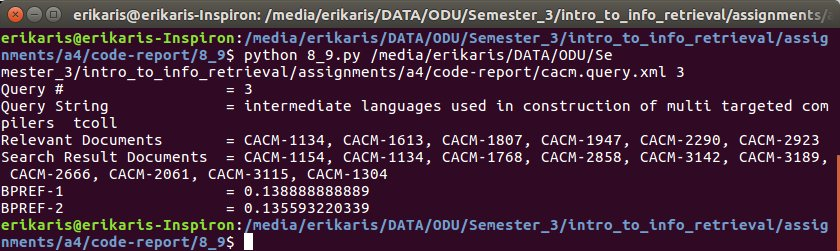
\includegraphics[scale=0.6]{89_output}}
	\centering
	\caption{BPREF values for query no. 3}
	\label{fig:89_output}
\end{figure}

From figure \ref{fig:89_output}, we can see that the 2 formulations of BPREF values give the similar value that are only slight different in the number of decimal places.  The code to generate the BPREF values can be found on listing \ref{lst:89}

\begin{lstlisting}[language=python, caption={Code for calculating BPREF values}, label={lst:89}]
#!/usr/bin/python

import errno
import os
from optparse import OptionParser
from lib.galago import GalagoRank

if __name__ == '__main__':
parser = OptionParser(description='Generate a ranking using Galago')
parser.set_usage(parser.get_usage().replace('\n', '') + ' <xml_file_input> [q1 ... qn]')
parser.add_option('-g', '--galago', dest="galago_bin", default='/media/erikaris/DATA/ODU/Semester_3/intro_to_info_retrieval/galago/galago-3.10-bin/bin/galago',
help='Galago "home" directory')
parser.add_option('-d', '--document', dest="document_dir", default='/media/erikaris/DATA/ODU/Semester_3/intro_to_info_retrieval/assignments/a4/code-report/cacm',
help='Document directory to be indexed')
parser.add_option('-j', '--judgements', dest="judgements_file", default='/media/erikaris/DATA/ODU/Semester_3/intro_to_info_retrieval/assignments/a4/code-report/cacm.rel',
help='File .rel as galago eval judgments')
parser.add_option('-r', '--result', dest="result_count", default='10', help='Number of result')

(options, args) = parser.parse_args()
options = vars(options)

if len(args) < 2:
parser.print_help()
exit()


out_dir = os.path.abspath('output')

try: os.makedirs(out_dir)
except OSError, e:
if e.errno != errno.EEXIST: raise

index_dir = os.path.join(os.path.pardir, 'index')
xml_query_file = os.path.abspath(args[0])
json_query_file = os.path.join(out_dir, 'query.json')
rel_file = os.path.join(out_dir, 'result.rel')
res_file = os.path.join(out_dir, 'result.res')
eval_file = os.path.join(out_dir, 'result.eval')

q_ids = []
if len(args) > 1:
q_ids = args[1:]

galago = GalagoRank(options['galago_bin'], options['judgements_file'])
if galago.index(options['document_dir'], index_dir):
for q_id in q_ids:
json_query = galago.build_json_input(xml_query_file, json_query_file, q_id)

rel_docs = galago.get_relevance_docs(q_id)
res_docs = galago.search(index_dir, json_query_file, res_file, options['result_count'])

galago.eval(options['judgements_file'], res_file, eval_file)

print 'Query #                  = {}'.format(json_query['number'])
print 'Query String             = {}'.format(json_query['text'])
print 'Relevant Documents       = {}'.format(', '.join(rel_docs))
print 'Search Result Documents  = {}'.format(', '.join(res_docs))
print 'BPREF-1                  = {}'.format(galago.get_bpref_1(rel_docs, res_docs))
print 'BPREF-2                  = {}'.format(galago.get_bpref_2(rel_docs, res_docs))


\end{lstlisting}

\medskip

\bibliographystyle{unsrt}%Used BibTeX style is unsrt
\bibliography{biblio}

\end{document}
